\section{Tool Hallucination and Reliability Evaluation}
\subsection{Tool Hallucination}


\begin{figure}[htbp]
    % \setlength{\belowcaptionskip}{-12pt} 
    \centering
    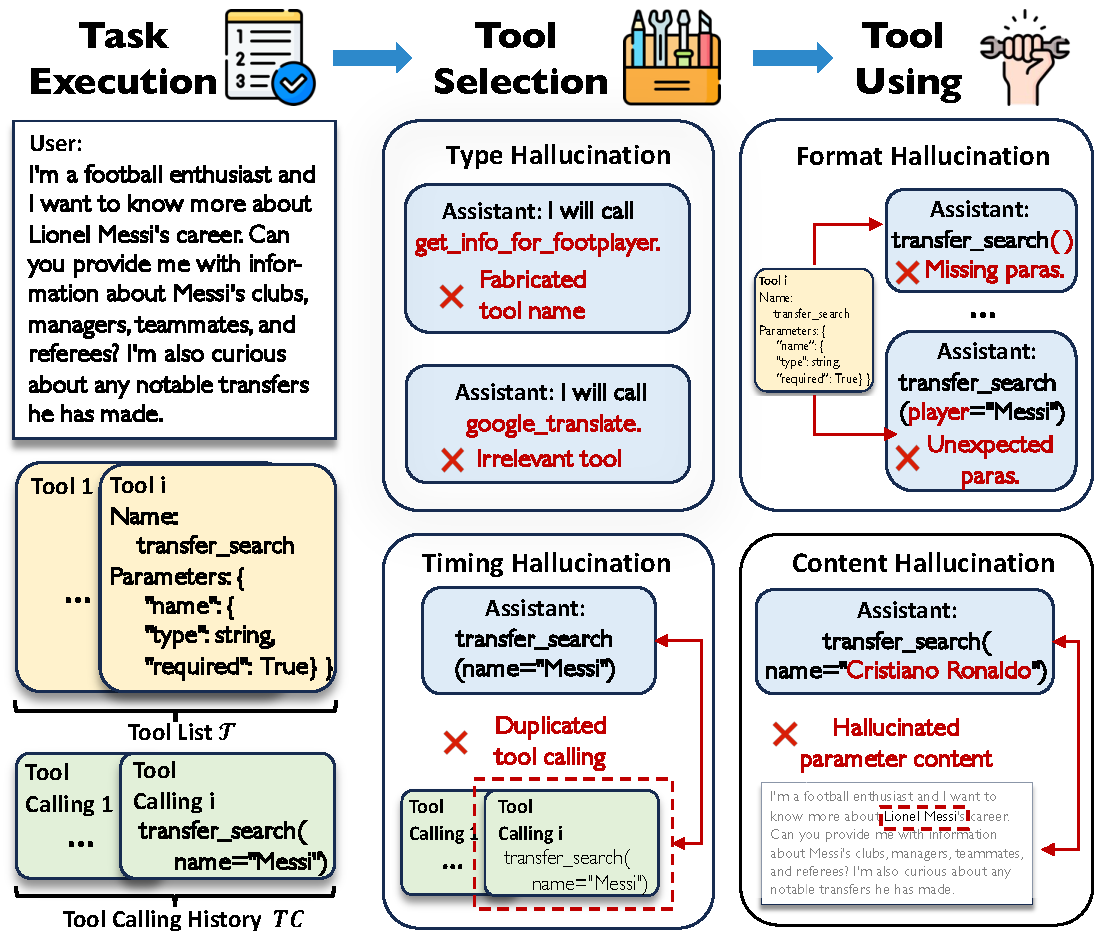
\includegraphics[width=0.48\textwidth]{figs/hallucination_type.pdf}
    \vspace{-6mm}
    \caption{Different types of tool hallucination.}
    % \vspace{-4mm}
    \label{fig:hallucination_type}
\end{figure}

\begin{figure}[t!]
    \centering
    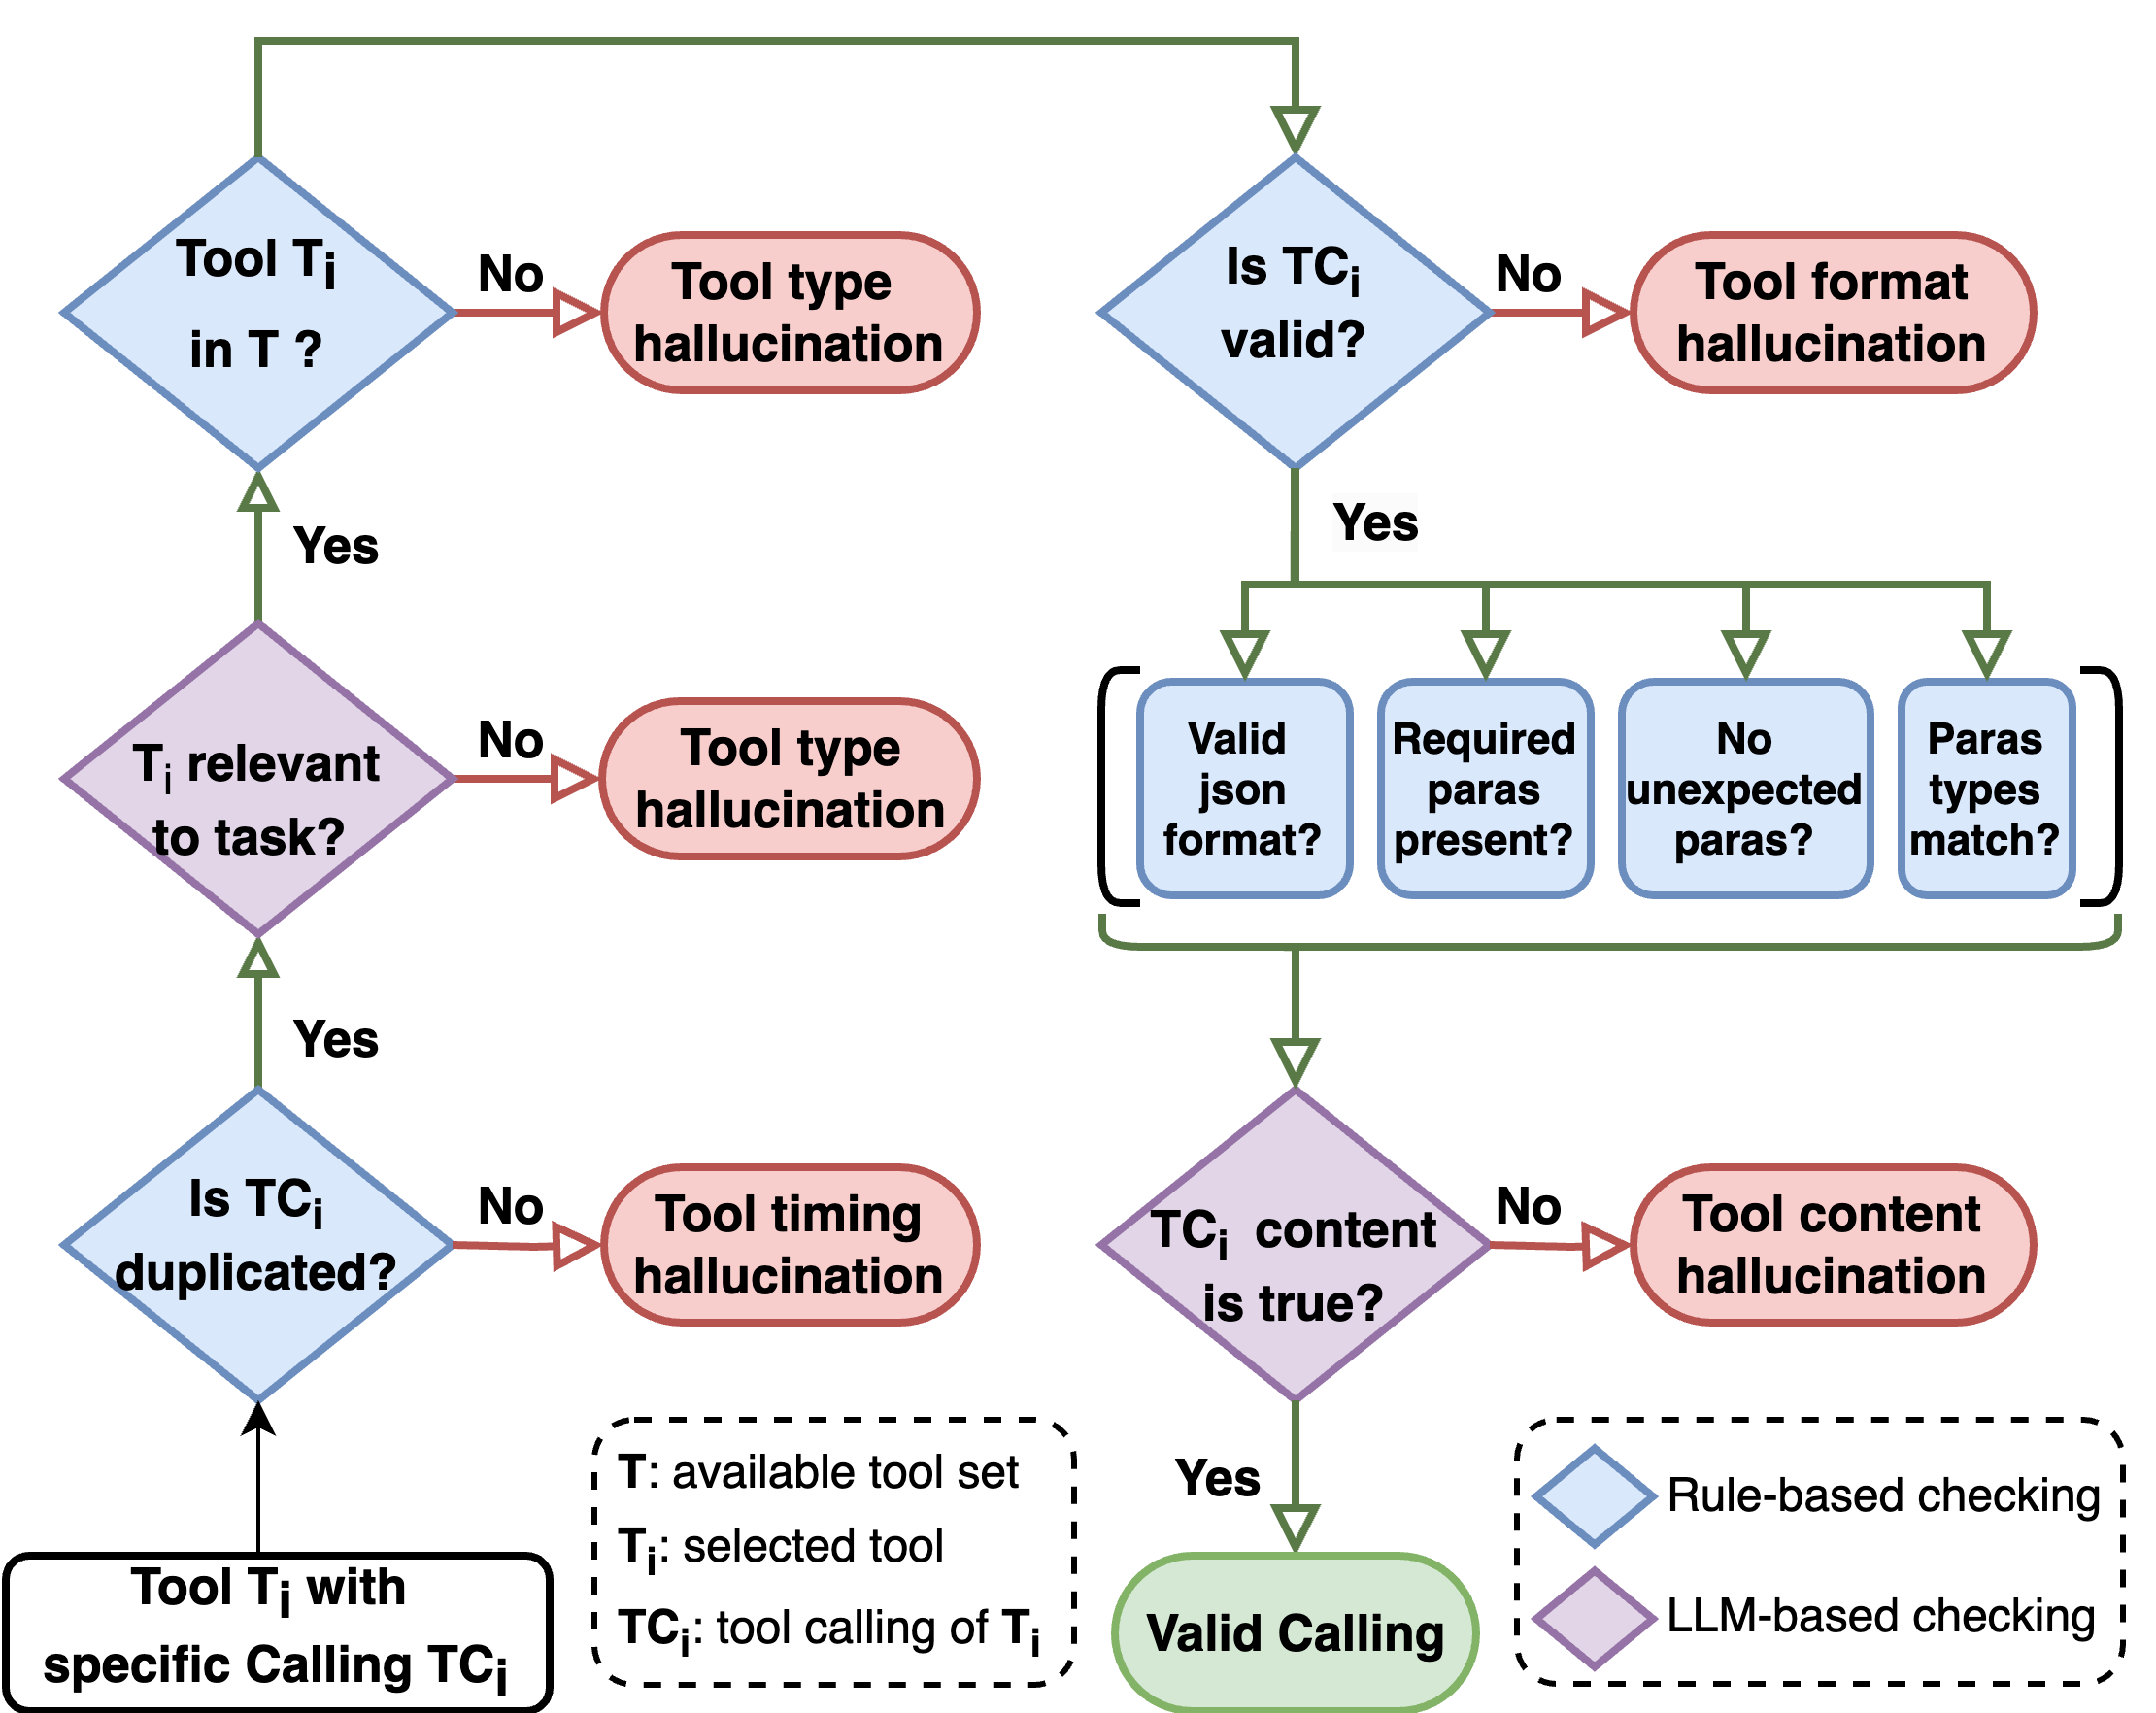
\includegraphics[width=\linewidth]{figs/tool_hallu.png}
    \vspace{-4mm}
    \caption{Evaluation process of tool hallucination.}
    % \vspace{-4mm}
    \label{fig:hallu_eval}
\end{figure}

With the emergence of intelligent agent frameworks like AutoGPT and MetaGPT~\cite{hong2024metagpt}, LLMs now demonstrate enhanced capabilities in real-world interactions through tool use. However, when LLMs interface with external environments via these tools, hallucinations during tool execution can directly affect real-world systems. 

We view tool calling as a decision-making action. When the conditions for making a decision are not met or when the decision fails, it can result in unexpected hallucinations. We categorize the tool hallucination into two major types: 

\textbf{Tool selection hallucination} occurs when the model either selects an inappropriate tool or calls a tool at the wrong time. This category can be further divided into two subtypes: 

\begin{itemize}
    \item \textbf{\textit{Tool type hallucination}} indicates that the model either invokes a tool that is unrelated to the task or fabricates a tool that does not exist in the available tool set.
    \item \textbf{\textit{Tool timing hallucination}} involves errors related to the sequence of tool calling. Specifically, this form of hallucination occurs when the model calls the same tool repeatedly with identical inputs and outputs, indicating that the tool should not have been called again at that point in the task process.
\end{itemize}



\textbf{Tool usage hallucination} pertains to errors in how the model uses a tool after selecting it. This category includes:
\begin{itemize}
    \item \textbf{\textit{Tool format hallucination}} refers to errors in the structure or format of the tool’s usage, such as providing an invalid JSON format, using incorrect parameter names, omitting required parameters, or specifying parameters with values of the wrong data type.
    \item \textbf{\textit{Tool content hallucination}} represents cases where the specific content of the tool’s parameters is fabricated by the model, meaning that the input provided to the tool was not based on the user’s query but was instead invented by the model.
\end{itemize}

We then determine tool hallucinations and their types following the process in Figure~\ref{fig:hallu_eval}. To ensure comprehensive evaluation, we integrate rule-based methods with an LLM evaluator (GPT-4o).   Rule-based methods detect structural errors such as invalid JSON formats and missing parameters. However, assessing tool-task relevance and parameter authenticity requires deeper semantic understanding, which the LLM evaluator provides:  
\begin{itemize}
    \item \textbf{Tool-task relevance assessment.} The evaluator infers a tool’s intended function from its description and parameters, verifying alignment with the user query. It also detects errors in tool invocation timing, such as redundant or premature calls.
    \item \textbf{Parameter authenticity verification.} The evaluator checks whether tool parameters (e.g., user IDs, city names) are derived from the user’s input or fabricated. If a parameter lacks a clear basis in the query, it is classified as a hallucination.  
\end{itemize}

We design structured prompts (Appendix~\ref{sec:prompt_check_relevance}, \ref{sec:prompt_check_content_hallucination}) to guide these evaluations. Human assessment shows that LLM-based evaluation achieves 92.7\% accuracy (Appendix~\ref{sec:human_eval}), closely aligning with expert judgments.  

To quantify hallucinations, we introduce the \textbf{tool hallucination rate}, measuring the proportion of hallucinated tool calls in a given task. For a task with \( N_{\text{total}} \) tool calls and \( N_{\text{hallucination}} \) hallucinated calls, we define:  
\begin{equation*}
H_{\text{sample}} = 
\begin{cases} 
\frac{N_{\text{hallucination}}}{N_{\text{total}}} & \text{if } N_{\text{total}} > 0, \\
0 & \text{otherwise.}
\end{cases}
\end{equation*}  
The task-level hallucination rate is computed as the average sample-level hallucination rate across all task instances, providing an overall measure of tool-use reliability.

% We then determine whether a specific tool calling is hallucinated and identify its type through the process outlined in Figure~\ref{fig:hallu_eval}. It's important to note that we rely not only on rule-based detection like format checking but also leverage LLMs (specifically, GPT-4o) as an evaluator to assess certain aspects of hallucinated tool calls. The LLM plays a crucial role in evaluating the relevance between the tool and the task, as well as determining whether the tool calling parameters are derived from the user's input or fabricated by the model. The evaluation prompts are shown in the Appendix~\ref{sec:prompt_check_relevance},\ref{sec:prompt_check_content_hallucination}.

% Through rigorous human evaluation, we find that the LLM-based automatic evaluation achieves an overall accuracy of 92.7\% (details in Appendix~\ref{sec:human_eval}). This indicates that the LLM evaluator can closely align with human judgment, particularly in determining the relevance of the tool to the task and verifying the origin of tool parameters.



% Consequently, we introduce the \textbf{tool hallucination rate}, a metric designed to capture the proportion of hallucinated tool callings over a set of tasks. This metric first calculates hallucination rates at the sample level—for individual task executions—then averages these rates across all samples to obtain a more comprehensive measure of overall tool hallucination behavior. For a given task, let \( N_{\text{total}} \) represent the total number of tool callings, and \( N_{\text{hallucination}} \) denote the number of hallucinated tool callings. The sample-level tool hallucination rate is defined as:

% \begin{equation*}
% H_{\text{sample}} = 
% \begin{cases} 
% \frac{N_{\text{hallucination}}}{N_{\text{total}}} & \text{if } N_{\text{total}} > 0, \\
% 0 & \text{if no tools were invoked.}
% \end{cases}
% \end{equation*}
% \begin{equation} H_{\text{overall}} = \frac{1}{N_{\text{samples}}} \sum_{i=1}^{N_{\text{samples}}} H_{\text{sample}, i} \end{equation}


% where \( N_{\text{samples}} \) is the total number of tasks in the evaluation set, 


\subsection{Reliability Evaluation}

% While tool hallucinations introduce erroneous executions, their impact extends beyond isolated failures. They contribute to increased decision-making costs, inefficient resource usage, and degraded task reliability. Therefore, evaluating LLM tool use requires a holistic perspective that accounts for both task success and tool efficiency. To capture this balance, we introduce two key metrics:
% 1) Reliable Pass Rate and 2) Benefit-Cost Utility. Together, these metrics provide a comprehensive view of LLM reliability in tool use, moving beyond simple task success rates to evaluate models in real-world, resource-constrained scenarios.


% \subsubsection{Reliable Pass Rate}

% \textit{Reliable Pass Rate} is the proportion of tasks that were successfully passed without hallucinated answers (we refer the readers to ToolBench paper for detailed pass rate evaluation; we use LLM to check if the answer is hallucinated, the prompt is shown in Appendix~\ref{sec:prompt_check_hallucinated_answer}).

In this section, we assess the reliability of tool use in LLMs by introducing two key metrics: \textbf{Reliable Pass Rate (RePR)} and \textbf{Benefit-Cost Utility}. Both metrics offer distinct insights into the model's ability to perform tasks efficiently and accurately while managing tool-related challenges such as hallucinations. The Reliable Pass Rate emphasizes the accuracy of task completion, focusing on the reduction of hallucinations, while the Utility metric incorporates both the success of the task and the associated costs, penalizing excessive tool usage and hallucinations.

\subsubsection{Reliable Pass Rate}

The Reliable Pass Rate (RePR) measures the proportion of tasks successfully completed without hallucinated responses. RePR subtracts the hallucinated outcomes from the standard pass rate, offering a clearer view of a model’s reliability in executing tasks without introducing errors. The formula for calculating RePR is:
$$
\text{RePR} = \text{Pass Rate} - \text{Task Hallucination Rate}.
$$
Here, Pass Rate refers to the proportion of tasks that are successfully completed (for detailed evaluation methods, please refer to the ToolBench paper~\cite{qin2023toolllm}), and Task Hallucination Rate quantifies the proportion of tasks affected by tool hallucinations. Importantly, tasks with an original pass rate of 0 are not considered as having result hallucinations to avoid repeated punishment.  Once tool hallucinations are identified, task hallucination is further assessed by using an LLM to verify whether the known hallucinated tool calls correlate with the final task result (for the prompt, refer to Appendix~\ref{sec:prompt_check_hallucinated_answer}). We also present a comparison between the original pass rate and our RePR metric in Figure~\ref{fig:repr}. We observe that, across different datasets, there are certain result hallucinations that are not directly identifiable by various evaluation models. As a result, our RePR metric is significantly lower than the pass rate.

\begin{figure}[htbp]
    \centering
    % 第一个子图
    \begin{subfigure}[b]{0.23\textwidth}
        \centering
        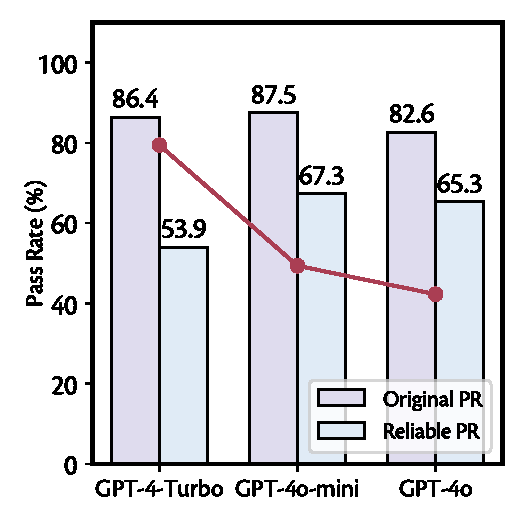
\includegraphics[width=\textwidth,trim=10 10 10 10,clip]{figs/pass_rate_models.pdf}
        % \caption{metric comparison over evaluators}
    \end{subfigure}
        \begin{subfigure}[b]{0.23\textwidth}
        \centering
        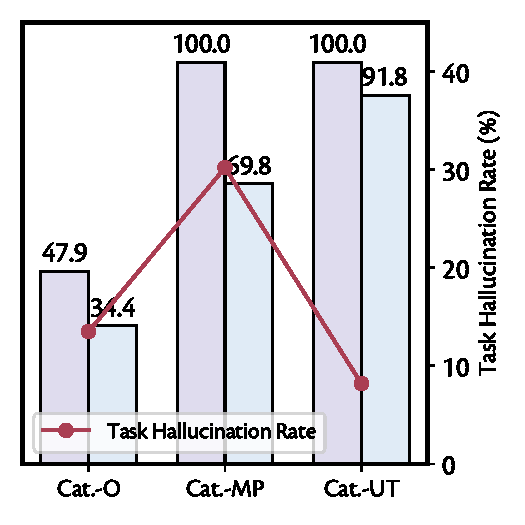
\includegraphics[width=\textwidth,trim=10 10 10 10,clip]{figs/pass_rate_items.pdf}
        % \caption{metric comparison over subsets}
    \end{subfigure}
    \vspace{-0.3cm}
    \caption{Metric comparison between reliable and original pass rate. O, MP, and UT represent the original, missing parameter, and unmatched tools subsets, respectively.}
    \label{fig:repr}
\end{figure}


\subsubsection{Benefit-Cost Utility}

The \textbf{Benefit-Cost Utility} takes a more holistic approach by evaluating both the task outcome and tool usage efficiency. The utility score is designed to reflect the overall quality of task execution, considering not only task success but also the penalties incurred from hallucinations and excessive tool calls. The formula for calculating the utility score is:
$$
\text{Utility} = R_{\text{task}} - P_{\text{tool}} - P_{\text{hallucination}},
$$
where \( R_{\text{task}} \) is the reward based on the task outcome (20 for success, 0 for failure), \( P_{\text{tool}} \) is the penalty for excessive tool usage (calculated as \( \min( \#(total\ tool\ calls) - \#(necessary\ tool\ calls), 10) \)), and \( P_{\text{hallucination}} \) is the penalty for hallucinations in the task (-10 for hallucination). 
Unlike RePR, which focuses solely on the task completion rate after excluding hallucinations, the Utility metric incorporates both the quality of the result and the efficiency of tool usage, making it a more comprehensive measure of tool reliability. It explicitly penalizes hallucinations and excessive tool calls, thus balancing the success rate with the cost of tool inefficiency and errors.

% In summary, while \textbf{RePR} primarily focuses on evaluating the model's ability to complete tasks correctly after excluding hallucinations, the \textbf{Utility} metric provides a broader measure that penalizes both hallucinations and inefficient tool use, offering a deeper insight into the overall reliability and cost-effectiveness of the model's tool interactions.








% \subsubsection{Benefit-Cost Utility}
% The \textbf{benefit-cost utility} serves as a reward-based metric that assigns a score to each task execution based on its outcome and the efficiency of tool usage. The utility captures the quality of the task result (success, failure, or hallucination) as well as the penalty for excessive tool calling. The scoring system is designed to incentivize both high task completion rates and efficient tool usage.


% The utility score for each task execution is therefore:

% \begin{equation}
% \text{Utility} = R_{\text{task}} - P_{\text{tool}}
% \end{equation}

% where $R_{\text{task}}$ is the reward based on task outcome (20 for success, 0 for failure, -10 for hallucination); $P_{\text{tool}}$ is the penalty for excessive tool callings, calculated as $\min( \#(total\ tool \ calls) - \#(necessary\ tool\ calls), 10)$.


\subsection{Construction of RelyToolBench}

To better evaluate tool hallucination and task reliability, we introduce RelyToolBench, which builds upon StableToolBench~\cite{guo2024stabletoolbench}. RelyToolBench extends the original test set by synthesizing two additional categories of subsets designed to simulate challenging conditions for the model. Both of the two categories are critical for evaluating the tool reliability of LLMs in real-world applications.  The dataset statistics are provided in the Table~\ref{tab:data_statistics}. Specifically, we generate two additional subsets:

\begin{itemize}
\item \textbf{Missing Parameter Subset}: This modification obscures certain parameters related to tool callings within the task. Specifically, this data is generated using LLMs to hide parameters within the tasks. This aims to simulate scenarios where crucial tool-related information is hidden, allowing us to evaluate the model’s ability to function effectively under incomplete information. The prompts can be found in the Appendix~\ref{sec:prompt_data_generation}.
\item \textbf{Unmatched Tools Subset}: We replace the tools specified in the task with irrelevant or mismatched tools. This modification tests the model’s ability to handle hallucinations arising from errors in tool selection, where the model may incorrectly identify or call the wrong tool for a given task.
\end{itemize}

% \begin{table}[ht]
% \centering
% \caption{\textbf{Data Statistics for ReleToolBench.} Ori: Original, MP: Missing Parameter, UT: Unmatched Tools.}
% \begin{tabular}{lcccc}
% \toprule
% \multirow{2.5}{*}{\textbf{Subset}} & \multirow{2.5}{*}{\textbf{Solvability}} & \multicolumn{3}{c}{\textbf{Count}} \\
% \cmidrule(lr){3-5}
%  & & \textbf{Ori} & \textbf{MP} & \textbf{UT} \\
% \midrule
% \multirow{2}{*}{I1 Instruction} 
%  & Solvable & 163 & -- & -- \\
%  & Unsolvable & -- & 99 & 163 \\
% \midrule
% \multirow{2}{*}{I2 Category} 
%  & Solvable & 124 & -- & -- \\
%  & Unsolvable & -- & 103 & 124 \\
% \midrule
% \multirow{2}{*}{I3 Instruction} 
%  & Solvable & 61 & -- & -- \\
%  & Unsolvable & -- & 60 & 61 \\
% \bottomrule
% \end{tabular}
% \label{tab:data_statistics}
% \end{table}



\begin{table}[ht]
% \begin{adjustbox}{width=\textwidth}
\centering
% \footnotesize
\caption{\textbf{Data Statistics for RelyToolBench.}}
\resizebox{\columnwidth}{!}{
\setlength\tabcolsep{3pt}
\renewcommand{\arraystretch}{0.8}
\begin{tabular}{cccccc}
\toprule

\multirow{2.5}{*}{\textbf{Category}} & \multirow{2.5}{*}{\textbf{Solvable}} & \multicolumn{3}{c}{\textbf{Subset}} & \multirow{2.5}{*}{\textbf{Total}}\\
\cmidrule(lr){3-5}
 % &  & \makecell{I1 \\Instruction} & \makecell{I2 \\Category} & \makecell{I3 \\Instruction}  &\\
 &  & I1-Inst. & I2-Cat. & I3-Inst.  &\\
\midrule
Original & \Checkmark & 163 & 124 & 61 & 348 \\
Miss Parameter & \XSolidBrush & 99 & 103 & 60 & 262 \\
Unmatched Tools & \XSolidBrush & 163 & 124 & 61 & 348 \\
\midrule
\quad Total & - & 425 & 351 & 182 & 958 \\
\bottomrule
\end{tabular}}
\label{tab:data_statistics}
% \end{adjustbox}
\end{table}



